% Created 2015-03-26 Thu 23:13
\documentclass[11pt]{article}
\usepackage[utf8]{inputenc}
\usepackage[T1]{fontenc}
\usepackage{fixltx2e}
\usepackage{graphicx}
\usepackage{longtable}
\usepackage{float}
\usepackage{wrapfig}
\usepackage{soul}
\usepackage{textcomp}
\usepackage{marvosym}
\usepackage{wasysym}
\usepackage{latexsym}
\usepackage{amssymb}
\usepackage{hyperref}
\tolerance=1000
\usepackage{methodshw, amsmath}
\providecommand{\alert}[1]{\textbf{#1}}

\title{8004 Homework 7}
\author{Nooreen Dabbish}
\date{\today}
\hypersetup{
  pdfkeywords={},
  pdfsubject={},
  pdfcreator={Emacs Org-mode version 7.9.3f}}

\begin{document}

\maketitle




\section{This is Problem 3 of Faraway (2006), Chapter 8.}
\label{sec-1}

The eggprod dataset concerns an experiment where six pullets were placed into each of 12 pens.
Four blocks were formed from groups of three pens based on location. Three treatments were
applied. The number of eggs produced was recorded.


\begin{verbatim}
library(faraway)
data(eggprod)
\end{verbatim}
\subsection{Fit a model for the number of eggs produced with the treatments as fixed effects and the blocks as random effects. Describe the estimated differences between the treatments.}
\label{sec-1-1}



pullet: a young hen, especially one less than one year old.

In the following model, y$_{\mathrm{ij}}$ is the number of eggs produced by the
\emph{i} th treatment on the \emph{j} th block, with i = 1, 2, and 3 and j = 1,
2, 3, and 4.

$$E(y_{ij}) = \beta_i,\,\text{ and
}y_{ij}=\beta_i+u_{j}+\epsilon_{ij}$$

We assume that 
\begin{itemize}
\item $u_{j}\overset{iid}\sim N(0,\sigma^2_u)$
\item the random error $\epsilon_{ij}\overset{iid}\sim
   N(0,\sigma^2_\epsilon)$
\end{itemize}


 



An overview of the dataset was performed and plots and descriptions are included in the
appendix. The \verb~summary()~ of our \verb.lme(eggs ~ 0+treat, random = ~1|block, data=eggprod, method=c("REML")). model of a means model terms gives
estimates for the means of treatments:


\begin{center}
\begin{tabular}{lrll}
 Treatment  &  Estimated Mean Eggs  &  Comparison  &  Difference  \\
\hline
 E          &               349.00  &  E-F         &  6.25 eggs   \\
 F          &               342.75  &  F-0         &  36.25 eggs  \\
 O          &               306.50  &  E-0         &  42.95 eggs  \\
\hline
\end{tabular}
\end{center}



That is, Treatment E's mean is 6.25 eggs greater than 
Treatment F. Treatment E's mean is 42.95 eggs greater than Treament
O. Finally, Treatment F's mean is 36.25 eggs greater than Treatment O.
\subsection{Test for the significance of the treatment.}
\label{sec-1-2}


In order to isolate the effect of treatment from the baseline means,
an intercept was added to the model. The new model may be written: 
$$E(y_{ij}) = \mu+ \beta_i,\,\text{ and }y_{ij} =\mu + \beta_i+u_{j}+\epsilon_{ij}$$
The assumptions made in part a) hold here.

The model matrix is now given by:



\[
\mathbf{X} = 
\begin{pmatrix}{}
  1 & 0 & 1 \\ 
  1 & 0 & 1 \\ 
  1 & 0 & 1 \\ 
  1 & 0 & 1 \\ 
  1 & 0 & 0 \\ 
  1 & 0 & 0 \\ 
  1 & 0 & 0 \\ 
  1 & 0 & 0 \\ 
  1 & 1 & 0 \\ 
  1 & 1 & 0 \\ 
  1 & 1 & 0 \\ 
  1 & 1 & 0 \\ 
  \end{pmatrix}
\]


We will use the likelihood ratio
test here, which tells us that given an MLE estimator $\hat{\theta}$
the quantity $-2(l(\hat{\theta} - l(\theta))$ follows a $\chi$$^2$
distribution with degrees of freedom equal to the dimensions of
$\theta$. The above ``l'' represents the log-likelihood function.

We compare the full model to a model with an intercept term only.
Therefore, our null hypothesis is that the differences in treatment 
represented by $\beta$$_2$ (Treatment F - Treatment E) and $\beta$$_3$
(Treatment O - Treatment E) are zero. Under the null hypothesis, these
terms are zero and the log-likelihood of the true $\theta$ our data
would given by a model with only an intercept term.


\begin{verbatim}
eggs.lme2 <- lme(eggs ~ 1 + treat, 
            random = ~1|block, data=eggprod, method=c("ML"))
eggs.lme3 <- lme(eggs ~ 1, random = ~1|block, data=eggprod, method=c("ML"))
LL2 <- logLik(eggs.lme2)
LL3 <- logLik(eggs.lme3)
W2 <- as.numeric(-2*(LL3-LL2))
W2
test <- qchisq(.95, 2)
\end{verbatim}

In the log-likelihood test performed above, a value of 
\texttt{8.4245} was obtained for -2log$\lambda$. This
compares to a .95 upper quantile of \texttt{5.9915} for
the $\chi$$^2$ dsitribution with df=2. Since our test value is more extreme, it
suggests the null hypothesis should be rejected, that the treatment 
effects are significant.
\section{This is Problem 4 of Faraway (2006), Chapter 8.}
\label{sec-2}


Data on the cutoff times of lawnmowers may be found in the dataset lawn. 3 machines were
randomly selected from those produced by manufacturers A and B. Each machine was tested twice
at low speed and high speed.


\begin{verbatim}
> library(faraway)
> data(lawn)
\end{verbatim}
\subsection{Fit a mixed effects model with manufacturer and speed as main effects along with their interaction and machine nested in manufacturer as random effects. Write down the formula for the model. In the summary output for the model, you will find that fixed manufacturer effect has zero degrees of freedom. Explain why this is so (check your model formula).}
\label{sec-2-1}


We write the model: $y_{ijk} = \alpha_i + \beta_j + \gamma_{ij} +
u_{ik} + \epsilon_{ijk}$ where y$_{\mathrm{ijk}}$ is the cut-off time of the
lawn mower from the ith (i=1,2) manufacturer at the jth speed (j=1,2)
of the kth type of machine of that manufacturer (k=1,2,3). 

We assume that 
\begin{itemize}
\item $u_{ik}\overset{iid}\sim N(0,\sigma^2_u)$
\item the random error $\epsilon_{ijk}\overset{iid}\sim
   N(0,\sigma^2_\epsilon)$
\end{itemize}









We run the following in R, using * to indicate an interaction term
and \verb,random=~1|manufact/machine, for the random effects term. There,
the slash indicates that machine is nested under manufact. The 1
indicates our assumption of constant/homogeneous variance:


\begin{verbatim}
lawn.lme <- lme(time ~ manufact + speed + manufact*speed, 
                random=~1|manufact/machine, data=lawn, method=c("REML"))

summary(lawn.lme)
\end{verbatim}

The complete output of \verb~summary(lawn.lme)~ is included in the
appendix. For readability, I am showing the Fixed effects table
illustrating that manufactB has 0 degrees of freedom (DF).


\begin{verbatim}
Fixed effects: time ~ manufact + speed + manufact * speed 
                     Value Std.Error DF   t-value p-value
(Intercept)      270.50000 12.200845 16 22.170595  0.0000
manufactB        -21.83333 17.254601  0 -1.265363     NaN
speedL           -60.33333  6.640831 16 -9.085208  0.0000
manufactB:speedL   2.66667  9.391554 16  0.283943  0.7801
\end{verbatim}

The manufacturer effect has zero degrees of freedom because this
factor is completely determined by the machine. That is, given a
machine of type ``m5'' for example, the manufacturer is B. The
information contained in the manufacturer factor (A or B) is already
contained in the machine factor (m1/m2/m3 or m4/m5/m6).
\subsection{Show why the manufacturer term may be removed from the fixed effect part of the model.}
\label{sec-2-2}


In order to determine if the term may be removed from the model, we
compare the models by ANOVA with and without the manufact factor and 
do not obtain a significant result. To validate this result, we
perform likelihood ratio testing.



\begin{verbatim}

lawn.lme <- lme(time ~ manufact + speed + manufact*speed, 
                random=~1|manufact/machine, data=lawn, method=c("ML"))

lawn.lme2 <- lme(time ~ speed, 
                 random=~1|manufact/machine, data=lawn, method=c("ML"))

anova(lawn.lme,lawn.lme2)
\end{verbatim}

\begin{verbatim}
           Model df      AIC      BIC    logLik   Test  L.Ratio p-value
 lawn.lme      1  7 204.9064 213.1528 -95.45319                        
 lawn.lme2     2  5 204.5690 210.4593 -97.28451 1 vs 2 3.662641  0.1602
\end{verbatim}

To validate the ANOVA result, we perform a log-liklihood test.


\begin{verbatim}

LL <- logLik(lawn.lme)
LL2 <- logLik(lawn.lme2)
W2 <- as.numeric(-2*(LL2-LL))
test2 <- qchisq(.95,2)
\end{verbatim}


The value of -2log$\lambda$ obtained in our test was
\texttt{3.6626}, which is less than the .95
quantile of the $\chi$$^2$ distribution with df=2, 
\texttt{5.9915}. This means the null is more
likely and shows that we should accept the null hypothesis that the 
the main effect manufacturer term and interaction parameters are 0. 
\subsection{Determine if the manufacturer term can be removed from the random part of the model.}
\label{sec-2-3}
\subsubsection{Significance of contribution of entire random term}
\label{sec-2-3-1}

We first test the removal of the entire random term (Machine type by
Manufacuturer) from the model.



\begin{verbatim}

lawn.lm4 <- lm(time ~ speed, data=lawn)

lawn.lme2 <- lme(time ~ speed, 
                 random=~1|manufact/machine, data=lawn, method=c("ML"))  

anova(lawn.lme2,lawn.lm4)
\end{verbatim}

\begin{verbatim}
 [1] 3.6626
 [1] 5.9915
           Model df      AIC      BIC     logLik   Test  L.Ratio p-value
 lawn.lme2     1  5 204.5690 210.4593  -97.28451                        
 lawn.lm4      2  3 211.9854 215.5196 -102.99271 1 vs 2 11.41639  0.0033
\end{verbatim}


\begin{verbatim}
LL <- logLik(lawn.lm4)
LL2 <- logLik(lawn.lme2)
W2 <- as.numeric(-2*(LL-LL2))
test2 <- qchisq(.95,5)
\end{verbatim}

Log liklihood testing for the removal of the entire random term
supported the significant ANOVA conclusion (p = 0.0033). A
-2log$\lambda$ value of \texttt{11.4164} was obtained, which is 
larger than the reference value of  the .95 quantile of the $\chi$$^2$
distribution with df=5 (5 because there are six machines, minus one
for overall), \texttt{11.0705}.
\subsubsection{Removal of nesting of manufact from random term.}
\label{sec-2-3-2}



\begin{verbatim}

lawn.lme2 <- lme(time ~ speed, 
                 random=~1|manufact/machine, data=lawn, method=c("ML"))  
lawn.lme3 <- lme(time ~ speed, 
                 random=~1|machine, data=lawn, method=c("ML"))  


anova(lawn.lme2,lawn.lme3)
\end{verbatim}

\begin{verbatim}
 [1] 11.4164
 [1] 11.0705
           Model df      AIC      BIC    logLik   Test   L.Ratio p-value
 lawn.lme2     1  5 204.5690 210.4593 -97.28451                         
 lawn.lme3     2  4 202.7968 207.5090 -97.39840 1 vs 2 0.2277637  0.6332
\end{verbatim}


\begin{verbatim}
LL3 <- logLik(lawn.lme3)
LL2 <- logLik(lawn.lme2)
W2 <- as.numeric(-2*(LL3-LL2))
test2 <- qchisq(.95,1)
\end{verbatim}

Log liklihood testing for the removal of the nested manufact component
of the random term
supported the NOT significant ANOVA conclusion (p = 0.6332). A
-2log$\lambda$ value of \texttt{0.2278} was obtained,
which is much smaller than the reference value of  the .95 quantile 
of the $\chi$$^2$ distribution with df=1 
(1 because one parameter is being tested), 
\texttt{3.8415}. So, the manufact nesting can be
removed from the random effects term.
\section{Appendix: Tangled R Code}
\label{sec-3}


\lstinputlisting{DabbishHW7.R} 
\section{Appendix: Additional and preliminary analysis of eggprod}
\label{sec-4}


Looking at the actual eggprod dataset proved useful (it is relatively
small):


\begin{center}
\begin{tabular}{lrr}
 O  &  1  &  330  \\
 O  &  2  &  288  \\
 O  &  3  &  295  \\
 O  &  4  &  313  \\
 E  &  1  &  372  \\
 E  &  2  &  340  \\
 E  &  3  &  343  \\
 E  &  4  &  341  \\
 F  &  1  &  359  \\
 F  &  2  &  337  \\
 F  &  3  &  373  \\
 F  &  4  &  302  \\
\end{tabular}
\end{center}



 
Additionally, boxplots Egg Production as a function of Treament and
Block were examined, as well as interaction plots. The boxplot of Egg
Production by Treatment shows that while Treatments E and F are
largely overlapping, Treatment O has a much lower mean and takes
lower values, completely non-overlapping with Treatment E.



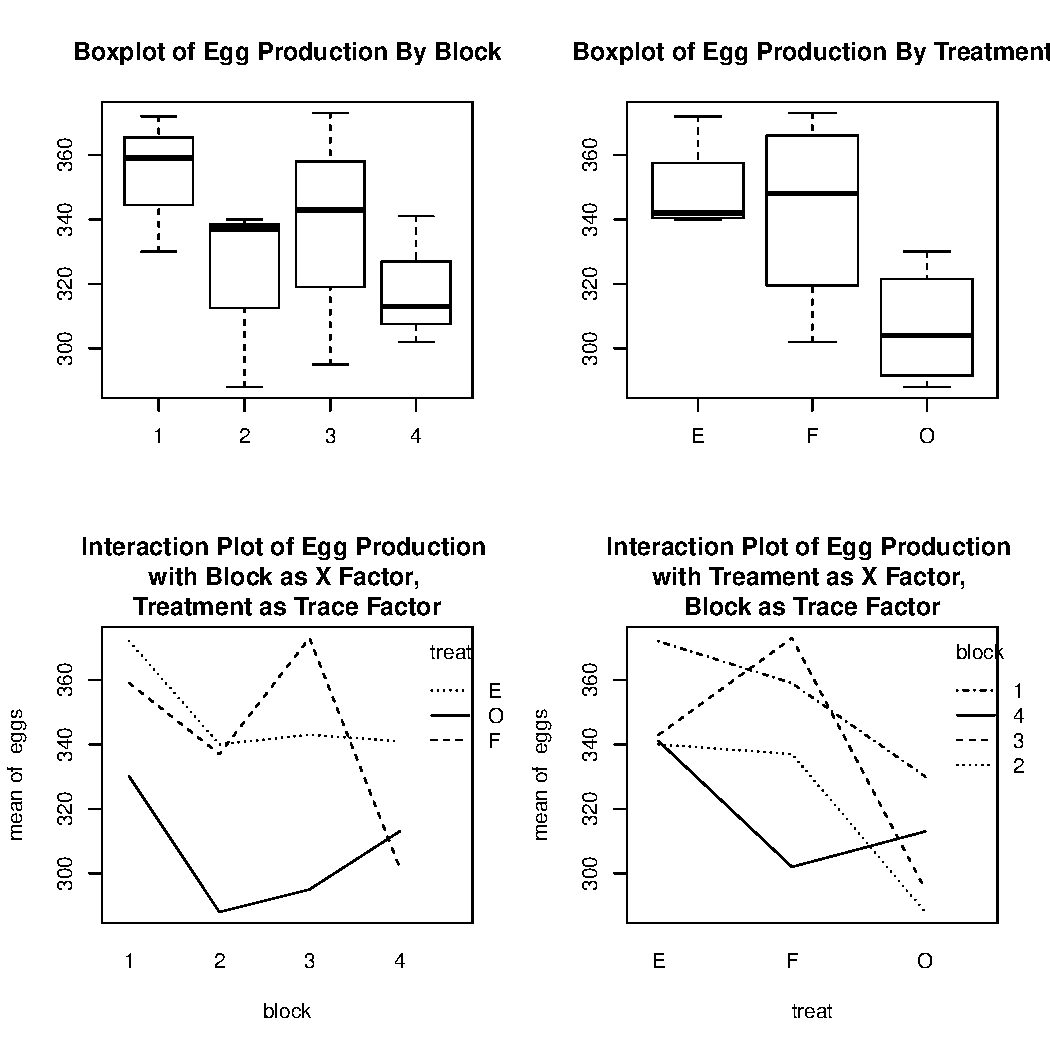
\includegraphics[width=.9\linewidth]{eggprod1.pdf}
\section{Appendix: Additional and preliminary analysis of lawn}
\label{sec-5}
\subsection{Prelimary analysis}
\label{sec-5-1}


The lawn data were plotted as boxplots of cut-off times versus
machine, speed, and manufacturer. The most striking observation was
that the cut-off times for speed ``H'' were much higher than speed ``L''.
In fact, the two box plots were non-overlapping. Means in the By
Machine boxplot appeared to vary, but all boxplots overlapped.

Interaction plots of cut-off times looking for an interaction between
manufacturer and speed show absolutely parallel lines, suggesting
there is no interaction.


\begin{figure}[htb]
\centering
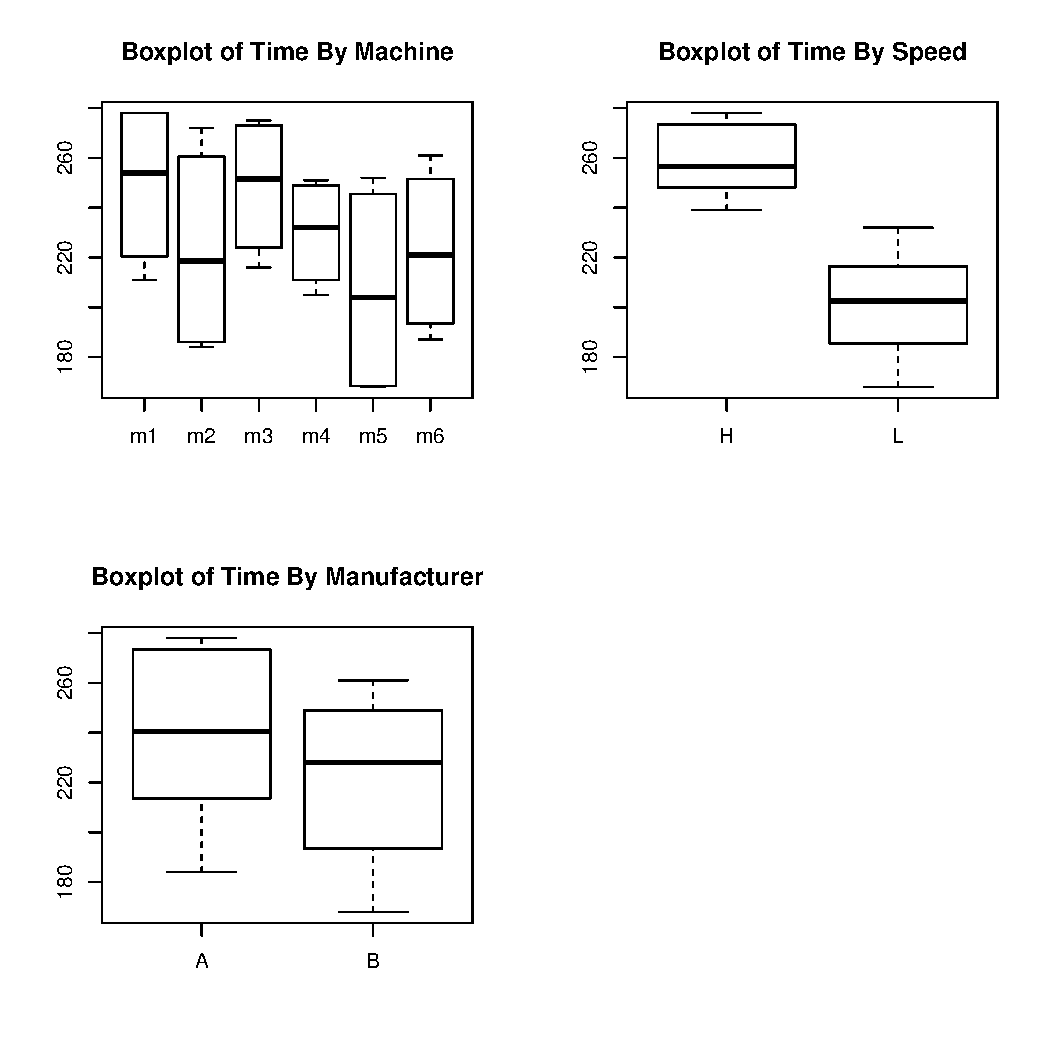
\includegraphics[width=.9\linewidth]{lawnplots.pdf}
\caption{Boxplot and Interaction plots for eggprod Boxplots of the lawn dataset}
\end{figure}


\begin{figure}[htb]
\centering
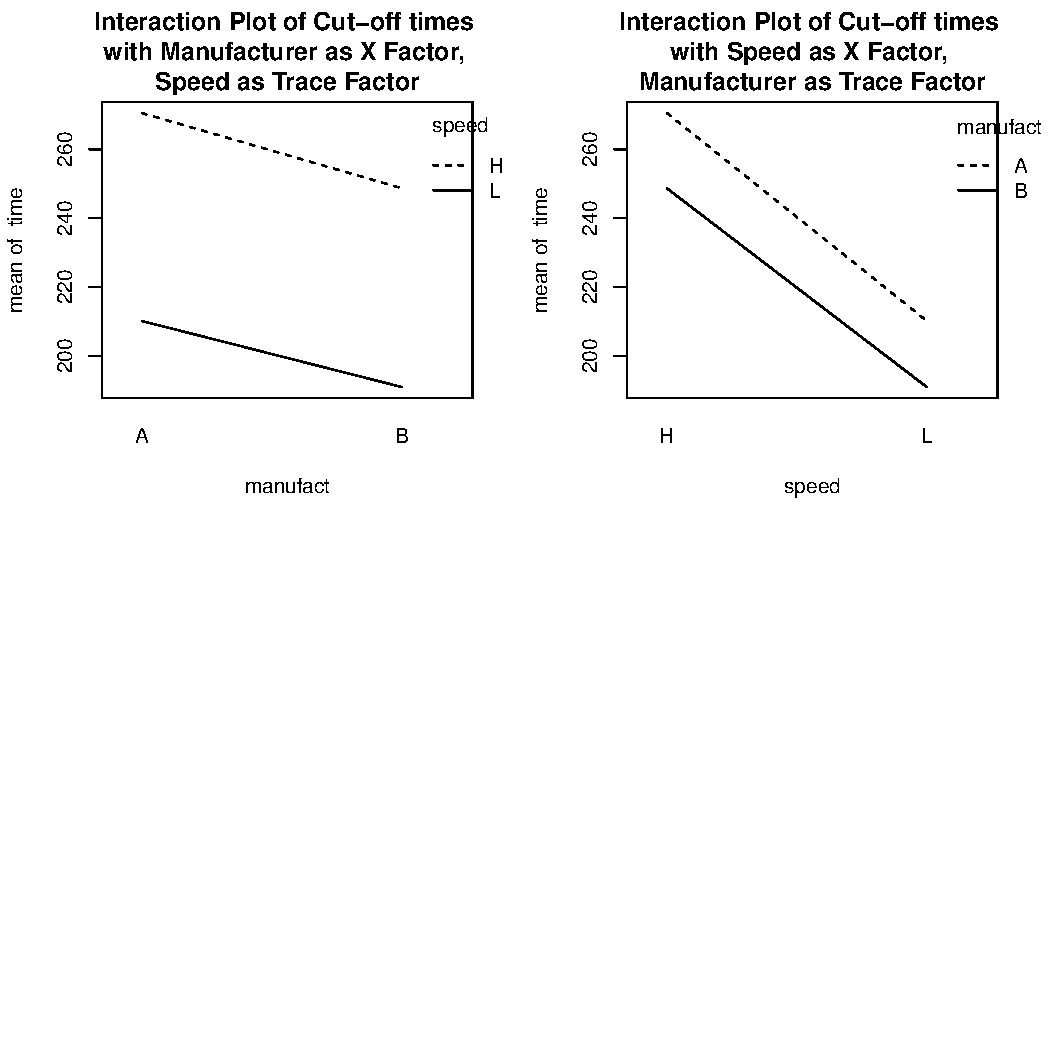
\includegraphics[width=.9\linewidth]{lawnplots2.pdf}
\caption{Interaction plots for Lawn}
\end{figure}
\subsection{Complete output of summary(lawn.lme)}
\label{sec-5-2}



\begin{verbatim}
Linear mixed-effects model fit by REML
 Data: lawn 
       AIC      BIC    logLik
  182.3651 189.3352 -84.18254

Random effects:
 Formula: ~1 | manufact
        (Intercept)
StdDev:    8.854442

 Formula: ~1 | machine %in% manufact
        (Intercept) Residual
StdDev:    12.05104 11.50226

Fixed effects: time ~ manufact + speed + manufact * speed 
                     Value Std.Error DF   t-value p-value
(Intercept)      270.50000 12.200845 16 22.170595  0.0000
manufactB        -21.83333 17.254601  0 -1.265363     NaN
speedL           -60.33333  6.640831 16 -9.085208  0.0000
manufactB:speedL   2.66667  9.391554 16  0.283943  0.7801
 Correlation: 
                 (Intr) mnfctB speedL
manufactB        -0.707              
speedL           -0.272  0.192       
manufactB:speedL  0.192 -0.272 -0.707

Standardized Within-Group Residuals:
       Min         Q1        Med         Q3        Max 
-1.0908529 -0.6739824 -0.1291112  0.6660725  1.5405034 

Number of Observations: 24
Number of Groups: 
             manufact machine %in% manufact 
                    2                     6 
Warning message:
In pt(-abs(tTable[, "t-value"]), tTable[, "DF"]) : NaNs produced
\end{verbatim}

\end{document}
